\makeatletter\let\ifGm@compatii\relax\makeatother
           

\documentclass[xcolor=dvipsnames]{beamer}

\usetheme{PaloAlto}

\usecolortheme{dolphin}

\setbeamertemplate{theorems}[numbered]

\setbeamertemplate{footline}[frame number]

\usepackage{epsf}
\usepackage{amsmath}
\usepackage{amsfonts}
\usepackage{amssymb}
\usepackage{amsthm}
\usepackage{latexsym}
\usepackage{mathrsfs}
\usepackage{amscd}
\usepackage{tikz}


\newcommand{\ms}[1]{\mathscr{#1}}               % Script

% Items done in default theorem style
\newtheorem*{thm}{Theorem}
\newtheorem*{prop}{Proposition}
\newtheorem*{lem}{Lemma}
\newtheorem*{Wconj}{Weinstein Conjecture}
\newtheorem*{conj}{Conjecture}
\newtheorem*{cor}{Corollary}


% Items done in definition style
\theoremstyle{definition}
\newtheorem*{defn}{Definition}
\newtheorem*{exmp}{Example}
\newtheorem*{prob}{Prob}
\newtheorem{ques}{Question}
\newtheorem*{question}{Question}
\newtheorem*{rem}{Remark}


\newcommand{\veps}{\varepsilon} 

\newcommand{\R}{\mathbb{R}}

\newcommand{\Z}{\mathbb{Z}}

\newcommand{\N}{\mathbb{N}}

\newcommand{\T}{\mathbb{T}}


\DeclareMathOperator{\dR}{dist}

\providecommand{\abs}[1]{\left\lvert#1\right\rvert}        % Absolute value

\providecommand{\norm}[1]{\left\lVert#1\right\rVert}       % Norm 
                                
\providecommand{\del}{\partial}

\newcommand{\vp}{\varphi}
\newcommand{\Lop}{L^1[-\pi,\pi]}
\newcommand{\Lor}{L^1(\R)}
\newcommand{\Ltp}{L^2[-\pi,\pi]}
\newcommand{\Fej}{Fej\'{e}r\ }
\newcommand{\inner}[1]{\left<#1\right>}
\renewcommand{\d}{\delta}
\newcommand{\e}{\epsilon}
\renewcommand{\k}{\kappa}

\begin{document}



\raggedright

\title{A Complete Orthonormal Sequence for $\Ltp$}
\author{Jeffery Cavallaro}

\date{Math 231B \\ December 11, 2017}

\begin{frame}

\titlepage

\end{frame}

\begin{frame}
  \frametitle{Introduction}

  Question: Is $(\vp_n)$, where $\vp_n(x)=\frac{1}{\sqrt{2\pi}}e^{inx}$, a
  bi-infinite complete orthonormal sequence in $\Ltp$?

  \begin{itemize}

  \item Orthonormality
  \item Convolution
  \item Summability Kernels
  \item The \Fej Kernel
  \item $\norm{K_n\star f-f}_1\to0$
  \item $f\in\Lop$ and $\inner{f,\vp_n}_{L_2}=0\implies f\equiv0$
  \item $f\in\Ltp\implies f\in\Lop$ (H\"{o}lder)
  \item $(\vp_n)$ is complete
  \end{itemize}

\end{frame}



\begin{frame}
  \frametitle{Orthonormality}

  \begin{itemize}

  \item $\int_{-\pi}^{\pi}e^{inx}dx=\begin{cases}
  2\pi, & n=0 \\
  0, & n\in\Z-\{0\}
  \end{cases}$

  \item $\int_{-\pi}^{\pi}\vp_n(x)dx=\begin{cases}
  \sqrt{2\pi}, & n=0 \\
  0, & n\in\Z-\{0\}
  \end{cases}$

  \item $\inner{\vp_m,\vp_n}=\begin{cases}
  1, & m=n \\
  0, & m\ne n
  \end{cases}$

  \end{itemize}
  
\end{frame}

\begin{frame}
  \frametitle{Convolution}
  
  \begin{defn}[Convolution]
    Let $f,g\in\Lor$. The convolution of $f$ and $g$, denoted $f\star g$, is
      given by:
      \[(f\star g)(x)=\int_{-\infty}^{\infty}f(x-t)g(t)dt\]
  \end{defn}
  \begin{defn}[Convolution on the Circle]
    Let $f,g\in\Lor$ be $2\pi$-periodic. Convolution on the circle is given by:
    \[(f\star g)(x)=\frac{1}{2\pi}\int_{-\pi}^{\pi}f(x-t)g(t)dt\]
  \end{defn}

  Convolution is commutative: $f\star g=g\star f$

\end{frame}




\begin{frame}
  \frametitle{Convolution Example}

  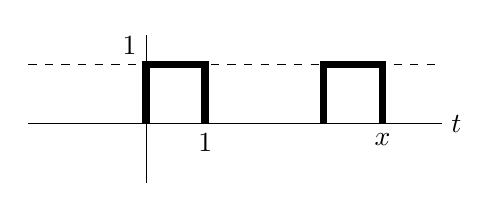
\begin{tikzpicture}[scale=0.75]
    \draw (-2,0) -- (5,0) node [right] {$t$};
    \draw (0,-1) -- (0,3/2);
    \draw [line width=1mm] (0,0) -- (0,1) -- (1,1) -- (1,0);
    \draw [line width=1mm] (3,0) -- (3,1) -- (4,1) -- (4,0);
    \node [below] at (1,0) {$1$};
    \node [below] at (4,0) {$x$};
    \draw [dashed] (-2,1) -- (5,1);
    \node [above left] at (0,1) {$1$};
  \end{tikzpicture}

  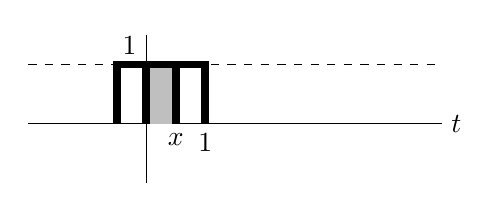
\begin{tikzpicture}[scale=0.75]
    \draw (-2,0) -- (5,0) node [right] {$t$};
    \draw (0,-1) -- (0,3/2);
    \draw [fill,color=lightgray] (0,0) rectangle (1/2,1);
    \draw [line width=1mm] (0,0) -- (0,1) -- (1,1) -- (1,0);
    \draw [line width=1mm] (-1/2,0) -- (-1/2,1) -- (1/2,1) -- (1/2,0);
    \node [below] at (1/2,0) {$x$};
    \node [below] at (1,0) {$1$};
    \draw [dashed] (-2,1) -- (5,1);
    \node [above left] at (0,1) {$1$};
  \end{tikzpicture}

  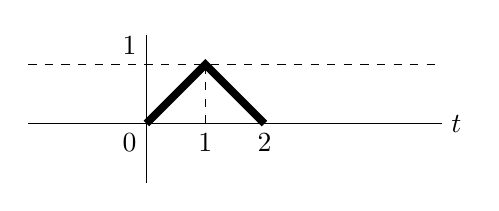
\begin{tikzpicture}[scale=0.75]
    \draw (-2,0) -- (5,0) node [right] {$t$};
    \draw (0,-1) -- (0,3/2);
    \draw [line width=1mm] (0,0) -- (1,1) -- (2,0);
    \draw [dashed] (1,0) -- (1,1);
    \node [below left] at (0,0) {$0$};
    \node [below] at (1,0) {$1$};
    \node [below] at (2,0) {$2$};
    \draw [dashed] (-2,1) -- (5,1);
    \node [above left] at (0,1) {$1$};
  \end{tikzpicture}
\end{frame}

\begin{frame}
  \frametitle{Summability Kernel}

  \begin{defn}[Summability Kernel]
    To say that a sequence $(\k_n)$ of $2\pi$-periodic continuous fuctions is
      a summability kernel means that $\k_n$ satisfies the following properties:
      \begin{enumerate}
      \item $\int_{-\pi}^{\pi}\k_n(t)dt=2\pi$
      \item $\int_{-\pi}^{\pi}\abs{\k_n(t)}dt\le M$ for some $M>0$ and all
          $n\in\N$
      \item $\int_{\d\le\abs{t}\le\pi}\abs{\k_n(t)}dt\to0$ for all $\d\in(0,\pi)$
    \end{enumerate}
  \end{defn}

  Note that the third property indicates that given a $\d>0$, For all $\e>0$
  there exists an $n$ sufficiently large such:
  \[2\pi(1-\e)<\int_{-\d}^{\d}\k_n(t)dt\le2\pi\]
  
\end{frame}

\begin{frame}
  \frametitle{The \Fej Kernel}
  
  \begin{defn}[Dirichlet Sequence]
    The Dirichlet sequence $(D_n)$ is given by:
    \[D_n(x)=\sum_{k=-n}^ne^{inx}\]
  \end{defn}

  \begin{defn}[\Fej Kernel]
    The \Fej kernel $(F_N)$ is given by:
    \[F_n(x)=\frac{1}{n+1}\sum_{k=0}^nD_k(x)\]
  \end{defn}

\end{frame}

\begin{frame}
  \frametitle{\Fej Kernel Forms}
  
  \begin{theorem}
    The following are equivalent forms of the \Fej kernel:
    \begin{enumerate}
    \item $F_n(x)=\frac{1}{n+1}\sum_{j=0}^n\sum_{k=-j}^je^{ikx}$

    \item $F_n(x)=\sum_{k=-n}^n\left(1-\frac{\abs{k}}{n+1}\right)e^{ikx}$

    \item $F_n(x)=\left(\frac{1}{N+1}\right)
    \frac{\sin^2\left[(n+1)\frac{x}{2}\right]}{\sin^2\left(\frac{x}{2}\right)}$
    \end{enumerate}
  \end{theorem}

\end{frame}

\begin{frame}
  \frametitle{$F_0$ through $F_5$}
  
  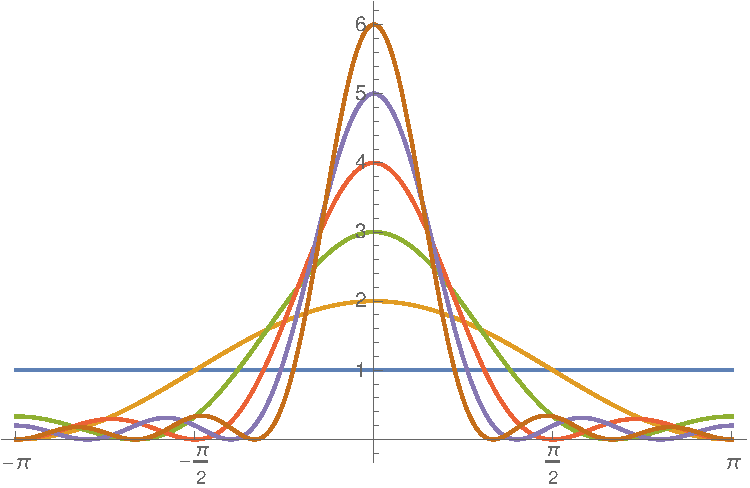
\includegraphics[scale=0.75]{plot}

\end{frame}




\end{document}
